\chapter{绪论}
\label{cha:intro}

\section{课题研究的目的和意义}
自第一台计算机出现以来,计算机软件安全成为计算机工程师不得花费心力思考的问题。在第一个蠕虫病毒出现之后,计算机的软件信息安全受到严重威胁。普通用户的计算机受到各种病毒和木马的威胁,其中包括大部分是通过网络传输到个人计算机中,通过修改程序的二进制代码,改变程序的执行流程,有的甚至被植入Shellcode代码,从而执行破坏或者窃取信息的代码,这是用户面临的软件程序的安全问题。

在当今互联网世界中,软件开发者的版权保护受到越来越多的关注,在二进制的层面上保护软件已经是很多软件生产公司最关注的问题之一,就算是Microsoft公司生产的Windows操作系统系列产品都会被技术水平较高的黑客破解\cite{芦天亮2020计算机病毒中的密码算法应用及防御方法综述},可见软件保护在当今互联网时代的难度之高,但是软件保护的意义不能小觑,很多商业软件依然给软件提供了各种注册方式,试图阻碍破解者获取软件正确序列号和逆向分析软件,其中包括通过网络验证、非对称加密RSA算法、机器注册码等方式。

类比于自然界植物用壳保护种子,计算机软件壳也是用来保护软件中的内容不被破解者非法修改。加壳软件在被保护软件中加入一段代码,并把原程序中代码执行区域中的代码加密、压缩,在程序正常运行时,被添加的代码会优先运行,为程序提供运行环境,包括整理堆栈、初始化CPU寄存器值等指令,最后对代码执行区域中的代码进行解密,转换为原代码后,最后将程序的执行权限交付给原程序。

软件盗版和篡改是世界面临的众所周知的威胁。已经进行了很多尝试来保护软件免受逆向工程和篡改。似乎软件开发人员和破解者之间正在进行一场战争,双方都希望随着时间的流逝相互竞争。审查了一些丰富的软件保护技术\cite{王欢2020构建高效},包括多块哈希方案,基于硬件的解决方案,校验和,混淆,防护,软件老化,加密技术和水印。所有这些技术都发挥了自己的作用,以保护软件免受恶意攻击。

软件保护在游戏行业也显得颇为重要,国内游戏软件两巨头腾讯和网易投入大量的人力资源对游戏软件加入反外挂机制,由于大部分网游都是运行在客户端,破解者可以通过分析二进制代码,使用ODDbg、IDA和WinDbg等反汇编工具对游戏进行动态或静态的反汇编\cite{徐君锋2017Android},技术较为程序的破解者通过分析汇编代码,是可以对整个游戏的流程进行细致分析,从而找出游戏中各种人物属性、技能、天赋在内存中的存放位置,最后可以使用C语言,对游戏进行远程内存注入,实现内存区域的控制,最后实现一个任意用户可用的游戏性外挂,这对当今依靠会员充值等方式盈利的公司是一个很大的打击,破解者甚至在分析游戏汇编代码后,可以构造网络游戏的网络包,直接对服务器发出伪造好的数据包,数据包中可能存放着购入金钱代码,直接对游戏进行充值,更有不法份子对这种修改软件进行售卖\cite{简容2019一种多层次的自动化通用},对游戏公司产生非常大的利益损失。

程序二进制混淆是软件开发人员和密码学专家长期以来一直感兴趣的话题。此处动机非常简单:找到一种方法,使我们可以为人们提供可以运行的程序,而无需他们弄清楚了程序是如何工作的,最后一部分必定会涉及很多内容\cite{钟林辉2020软件演化历史的逆向工程生成方法研究}。原则上,它包括从所使用的特定秘密算法的性质到可能会使用硬编码加密程序中的秘密信息等方面。

%对于一个简单的示例,请考虑一下例程:

%\begin{lstlisting}[language=C]
%// 检查密码,如果正确则打印出绝密信息
%SuperSecretPasswordProtectedStuff(string passwd) {
%if (password == “0x123”) {
%  print(“恭喜. 下面是一些重要的私人信息: ….\n”);
% } 
%else {
%  print(“密码错误.\n”);
% }
%}
%\end{lstlisting}

大多数程序都非常易于阅读,攻击者可能只是查看此程序即可恢复序列号密码\cite{徐君锋2017Android}。程序混淆的想法是,如果能够以某种方式阻止人们这样做,同时让他们拥有并在自己的计算机上运行的程序,那许多需要保护的软件都可以使用这种方式保护起来\cite{夏学云2019软件逆向工程技术分析}。

在现实世界的软件系统中,“混淆”通常是指一些临时技术的集合,这些技术将一些设计巧妙的程序变成许多GOTO代码组合,有时重要的常量会被切碎并分布在代码周围\cite{2020Malware}。该代码的某些部分甚至可以被加密,尽管是暂时的,因为解密密钥必须随程序一起提供才能真正运行\cite{2019Transforming}。

%^恶意软件作者都喜欢下图\ref{cha1:sub1:chunkcode}这种混淆。

%\begin{figure}[H]
%	\centering
%	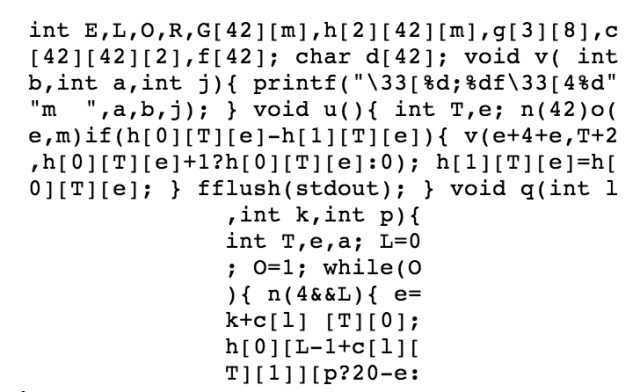
\includegraphics[width=0.7\textwidth]{chunkcode.png}\\
%	\caption{2013年C语言混淆大赛的获胜作品之一}
%	\label{cha1:sub1:chunkcode}
%\end{figure}
%尽管这些技术不错,但它们并不是真正的“不可破解”,甚至在我们想要的真正意义上也不能防止逆向工程。

只要有足够时间、精力和工具\cite{2018Analysis},人人都可以摆脱最常见的软件混淆技术\cite{2014A}。现有软件混淆的质量很差,是密码学家面临的问题。是否存在这样一个程序混淆加密器,用这样的混淆器来加密受保护的软件,同时要证明可保护所有需要保护的信息。如果能够做到这一点,它将拥有惊人的应用场景。股票交易者可以混淆其专有的交易算法\cite{2020Flow},然后将其发送到云端或者最终客户。产生的程序仍然可以正常工作\cite{0Black},但是客户永远不会学到“工作原理“的任何信息。在程序外看,程序就是一个黑匣子,而程序的内部将是各种混合机制和原有代码的融合\cite{2020A}。

%任何形式的复制保护都起源于密码学,Kerckhoffs原理是现在密码学中最重要的规则之一,它指出系统的安全性不应该取决于算法的秘密,而应该取决于密钥的秘密。因此,根据该方法构建的系统需要已知该机制,因为安全性仅基于排他性地基于可变密钥。许多加密方法都基于此原理。

因此,软件安全问题是普通用户和公司软件都不容忽视的问题,软件保护者需要开发出既能保证软件正常运行同时又避免被逆向者分析的软件保护程序,本文将针对软件保护程序进行相关技术的研究。


\section{国内外研究现状}
\label{cha1:sec:relatedworks}
在软件混淆加密技术领域,全球有诸多小组致力于此研究,也均在保证加密性能和运行性能下给出了出色的解决方案。
\subsection{国内研究现状}

浙江大学的高勇等人提出使用加密狗虚拟技术实现共享式工作平台,加密狗通常是USB记忆棒,改USB记忆棒连接到计算机上的端口以验证许可证\cite{秦飞2018逆向工程和}。使用USB加密狗运行的软件首先在启动后定期发送一个请求到I/O端口进行身份验证。一旦无法检索到与其的验证码,该程序就会自动终止,或者只能访问有限的功能\cite{Jeong2014Code}。加密狗尤其可以防止未授权的复制。原理本质上非常简单:没有加密狗,无法访问软件。现代硬件加密狗使用公私钥和对称机密过程,加密密钥不包含在应用程序的某个位置\cite{曾强2020Linux},而是安全地存储在Flash-ROM中,在其中它们无法被读出并仅用于加密和解密。除此之外,还有具有网络支持的加密狗,可以将其连接到网络中的任何计算机或服务器。许可证服务器应用程序正在此计算机上运行,并在网络中提供许可证。现在,受保护的应用程序将检查本地连接的加密狗或网络中的许可证服务器\cite{2019Analyzing},此外,还可以通过基于硬件,如CPU、主板和硬件驱动器等生成特殊的许可证密钥,讲软件许可证绑定到特定计算机,并将其存储在加密狗中。加密狗可以大大减少软件盗版,并且在数字版权管理中尤为有效,因为生成加密狗的非法副本非常困难。

在研究软件保护的初期,研究人员开发了一些相对有用的专业软件加密保护程序。但是,随着破解技术的发展,即使使用强大的加密算法,如Twofish,TEA,Blowfish以及CRC循环冗余校验和反调试技术的组合,坚固外壳ASProtect也可以通过使用免费的OllyDbg删除动态跟踪外壳后的反汇编代码。使用堆栈平衡原理在程序执行入口之前找到外壳,然后结合LoadPE工具的强大功能来导入表,导入地址表和重定位表。当前,VMProtect和驱动程序保护技术是保护软件的两种最重要的方法\cite{2020Call}。

国立台湾科技大学自动化与控制研究所使用AES算法对图像进行了加密试验,杨成雄教授提出了一种基于四维混沌系统的图像加密算法\cite{2017Access},以生成密钥并提高高级加密标准。通过使用现场可编程门阵列FPGA的流水线和并行计算功能来优化加密算法。首先,混沌系统用作加密算法的密钥生成器。接下来,在改进的高级加密标准中\cite{2018ORLIS},使用Spin-Sort和Cubic S-Box修改了ShiftRows和SubByres,并减少了加密次数。我们将加密算法和有线图像传输系统实现到基于ARM的SoC-FPGA。HPS软件在Linux上运行,用于控制FPGA加密算法和图像传输。


\subsection{国外研究现状}

比利时密码学家Vincent Rijmen和Joan Daemen开发了Rijndael分组密码\cite{段钢2003加密与解密}的子集,它们在AES选择过程中向NIST提交了提案\cite{2020Saturable}。Rijndael是具有不同密钥和块大小的密码家族。对于AES,NIST选择了Rijndael系列的三个成员\cite{0Compile2},每个成员的块大小为128位,但是具有三个不同的密钥长度:128、192和256位。AES已经被美国政府采用,现已在全球范围内使用\cite{2019Implementation}。它取代了1977年发布的数据加密标准DES。AES描述的算法是对称密钥算法,意味着同一密钥用于加密和解密数据。

麻省理工大学教授N. Sasirekha和M. Hemalatha提出了一种基于带Hadamard索引表准组加密和数字理论变换的有效安全代码方法\cite{2020Bacterial},以进行软件保护\cite{2020Detecting},此方法使用一种称为准组加密的新颖有效的加密技术对索引表进行加密。加密后,它与原始数据的相似性最小。准确有效地产生了复杂数字的密钥,这是逆向分析者难以识别原始数据。但是,准组加密在扩散纯文本的统计信息方面效率不高。因此,此方法使用链式Hadamard变换和数字理论变换将扩散与准群变换一起引入。实验结果基于时间成本和空间成本评估了所提出的加密方法的性能,并且观察到所提出的方法提供了重要的结果。



剑桥大学Barak等人提出了一种“不可区分性混淆程序”\cite{Kyu2020Clustering},简单可概括为如下内容:有两个程序$\mathit{C1}$和$\mathit{C2}$我们将它们描述为大小相似的电路,他们计算的功能相同,更具体地说,我们可以说它们具有完全相同的输入和输出行为,尽管它们在内部实现的方式可能非常不同,不可区分混淆的定义指出,应该对两个电路$\mathit{C1}$,$\mathit{C2}$进行混淆,以使没有有效的算法能够分辨$\mathit{Obf(C1)}$与$\mathit{Obf(C2)}$之间的差异。尽管这个想法是在多年前提出的,但实际上没有人知道如何构建这样的东西,称为那些“未解决的问题”之一。直到前年,情况仍然如此,直到IBM Research的一组作者基于多线程图的密码学新领域,提出了一种“候选构造”来构造这种混淆器\cite{2019White}。这个概念的另一个有趣的变种被称为萃取混淆$\mathit{Obf(EO)}$,这不仅意味着你不能分辨之间$\mathit{OBF(C1)}$和$\mathit{OBF(C2)}$,但是,如果你能区分这两种情况,那就可以找到一个输出值,$\mathit{C1}$和$\mathit{C2}$都将在该输入值上产生不同的输出。此外,其他工作表明$\mathit{IO}$和$\mathit{EO}$本质可以为常规程序提供必要好的混淆算法。

加利福尼亚大学Paul A. Cronce和Joseph M. Fontana等人提出一种将源代码转换为字节码来保护软件\cite{2019White}。他们的这种方式提供用于编程语言的语言规范,用于实现该语言的库,用于将该语言编译为字节码的编译器以及使用该库执行字节码的解释器\cite{2019Implementing};向软件发布者提供语言规范和说明,以及用于指导软件发布者如何从要保护的应用程序中选择代码部分以及如何准备所选代码部分和应用程序以在服务器上进行处理的说明,包括指示发布者在从应用程序中获取所选代码部分的相应位置创建数据结构;向服务器提供编译器、库、解释器和服务器应用程序,用于从发布者接收要保护的软件应用程序和准备好的代码选择部分。使用编译器将代码的选定部分编译为字节代码,将编译器生成的字节代码嵌入到应用程序中\cite{2018Code},并用解释程序调用替换数据结构,以调用代表已删除代码部分的适当字节代码模块的解释\cite{2018Method},从而使应用程序正确运行\cite{2018Securing},并在解释程序上运行经过混淆的代码部分和在应用程序中嵌入库和解释器以支持编译后的字节码的运行时解释,从而使所选段变得模糊\cite{2019Model}。




\section{本课题主要研究内容}

目前国内外的软件加密技术主要是使用硬件加密狗、高强度算法和使用字节码虚拟机等保护方式,以上方式都有各自的局限性,比如硬件保护方式虽然保护强度高,但是保护成本过高,每个程序的发型都需要适配一个USB硬件,不适合小型软件的发布,并且软件的运行过程由于需要插入USB设备,造成软件运行过于繁琐。高强度算法和字节码虚拟机等保护方式由于在运行过程中需要解码,所以存在软件运行效率急剧下降的问题。本文针对以上提出的问题,进行优化改进,保证了软件安全强度的前提下,尽可能提高软件的运行效率。

本文主要研究内容为:采用在反动态调试和反静态调试两个方面来防止未授权用户进行注册或者调试,反动态调试方面是对软件采用虚拟机加壳的方式,对软件进行打包,将大部分汇编代码转换为字节码,在运行时通过解释器翻译给操作系统,如果破解者不了解其中字节码和汇编代码的对应关系,将很难实现未授权注册行为;反静态调试是在已有的函数间基本块进行交换的静态保护算法基础上提出建立索引的方式对函数间基本块进行交换的静态保护算法,这种方式与剑桥大学研究内容的目标基本相同,都是对静态二进制代码进行混淆,加大IDA等静态反汇编工具的分析难度,建立索引的方式会在软件内部新增加一个节区,用来记录所有参与过函数块之间交换的块,在程序运行时,解释器会根据这个索引表进行软件的混淆机制恢复过程。

本文设计的虚拟机是一种解释执行系统与加利福尼亚大学提出的将源代码转换为字节码的原理相同,本文会提出一种基于虚拟机加壳的多样化Handler动态保护方法,在原有虚拟机保护的基础上,在二进制层面加大逆向者的分析难度,从而让软件得到更有效的保护。与解释执行语言中的虚拟机不同,本文设计的虚拟机是存在于每个可执行程序中的,所有被加密的软件都经过虚拟机加壳器的处理,其中的可执行硬编码都已经变成伪指令,即使破解者进入到虚拟机中跟踪虚拟机的解释器算法,由于每一套虚拟机的指令的不同,破解者将很难理解经过处理后的指令,破解者如果想正确逆向这样的软件,就必须对虚拟机的引擎进行深入的研究,通过不断的反复对比试验和猜测,最后形成伪指令和原始指令的对应关系,就像在破解一套摩尔斯电码但是不知道电码的字典一样,这样可以大大增加破解的难度和破译成本,也正是由于这种破解难度,虚拟机保护已经成为软件保护者的趋势。
